\documentclass[10pt,mathserif]{beamer}

\usepackage{graphicx,amsmath,amssymb,tikz,psfrag}

\input defs.tex

%% formatting

\mode<presentation>
{
\usetheme{default}
}
\setbeamertemplate{navigation symbols}{}
\usecolortheme[rgb={0.13,0.28,0.59}]{structure}
\setbeamertemplate{itemize subitem}{--}
\setbeamertemplate{frametitle} {
	\begin{center}
	  {\large\bf \insertframetitle}
	\end{center}
}

\newcommand\footlineon{
  \setbeamertemplate{footline} {
    \begin{beamercolorbox}[ht=2.5ex,dp=1.125ex,leftskip=.8cm,rightskip=.6cm]{structure}
      \footnotesize \insertsection
      \hfill
      {\insertframenumber}
    \end{beamercolorbox}
    \vskip 0.45cm
  }
}
\footlineon

%\AtBeginSection[] 
%{ 
%	\begin{frame}<beamer> 
%		\frametitle{Outline} 
%		\tableofcontents[currentsection,currentsubsection] 
%	\end{frame} 
%} 

%% begin presentation

\title{\large \bfseries Model-free Deep Reinforcement Learning -- Algorithms and Applications}

\subtitle{Reinforcement Learning Seminar Winter Semester 2018/2019}

\author{Fabian Otto\\[3ex]
Technische Universit\"at Darmstadt\\
Supervisor: Samuele Tosatto\\
Group: 16\\\vspace{15pt}
 
\includegraphics[height=0.8cm]{images/TU.png}\vspace{-20pt}}

\date{\today}

\begin{document}

\frame{
\thispagestyle{empty}
\titlepage
}

\AtEndDocument{
	\begin{frame}
		{\Large Thank you for your attention.\\
		Questions?\\}
		\vspace{50pt}
		\textbf{Contact:}\\
		Fabian Otto\\
		Technische Universit\"at Darmstadt, Computer Science Department\\
		fabian.otto@stud.tu-darmstadt.de
		
	\end{frame}
}

\begin{frame}
	\hspace*{0pt}\makebox[\linewidth][c]{%
		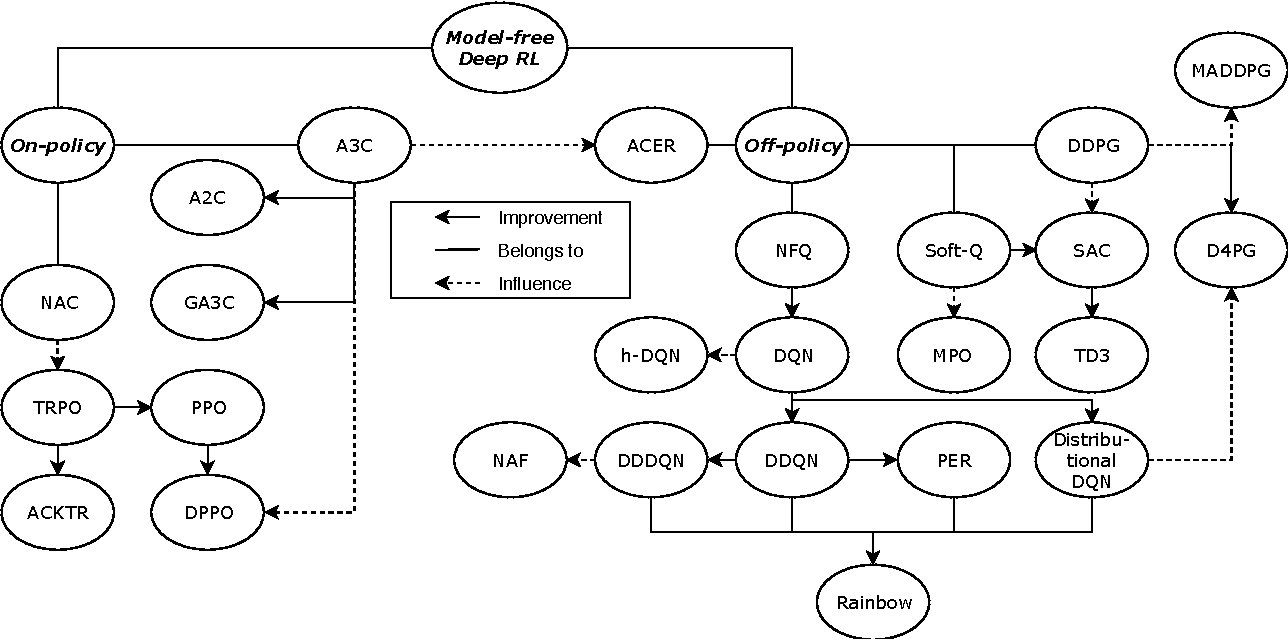
\includegraphics[width=1.1\textwidth]{images/tree_presentation2.pdf}
	}
\frametitle{Algorithms}

\end{frame}

\begin{frame}
\frametitle{Applications}
	\hspace*{0pt}\makebox[\linewidth][c]{%
		\begin{columns}[t]
				\column{.3\textwidth}
				\centering
				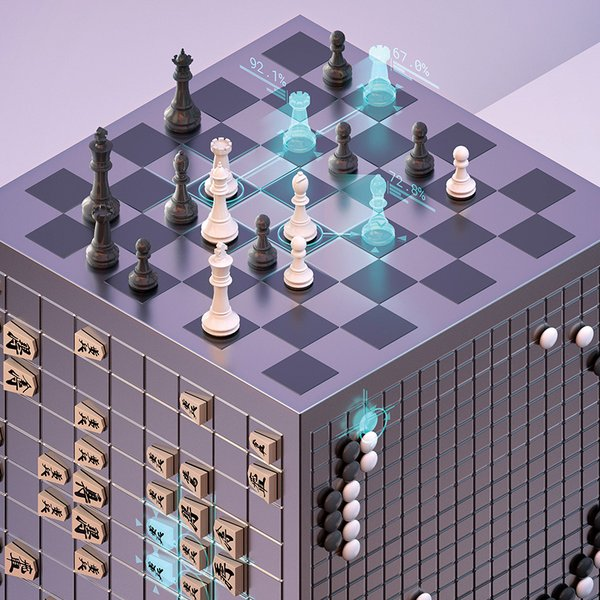
\includegraphics[scale=0.2]{images/Go.jpg}
				
\includegraphics[scale=0.05]{images/Dota2.jpeg}
				\column{.6\textwidth}
				\centering
				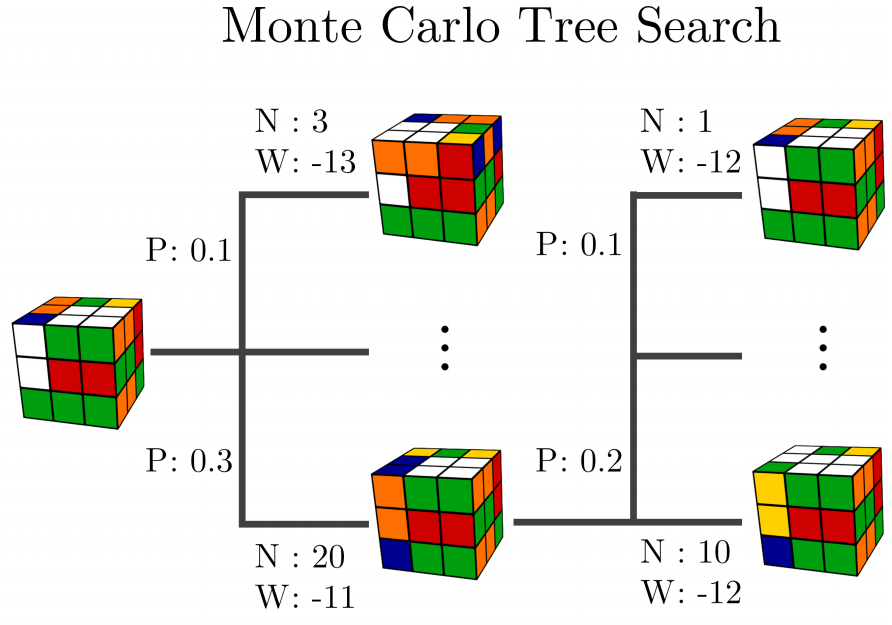
\includegraphics[scale=0.18]{images/Cube2.png}
				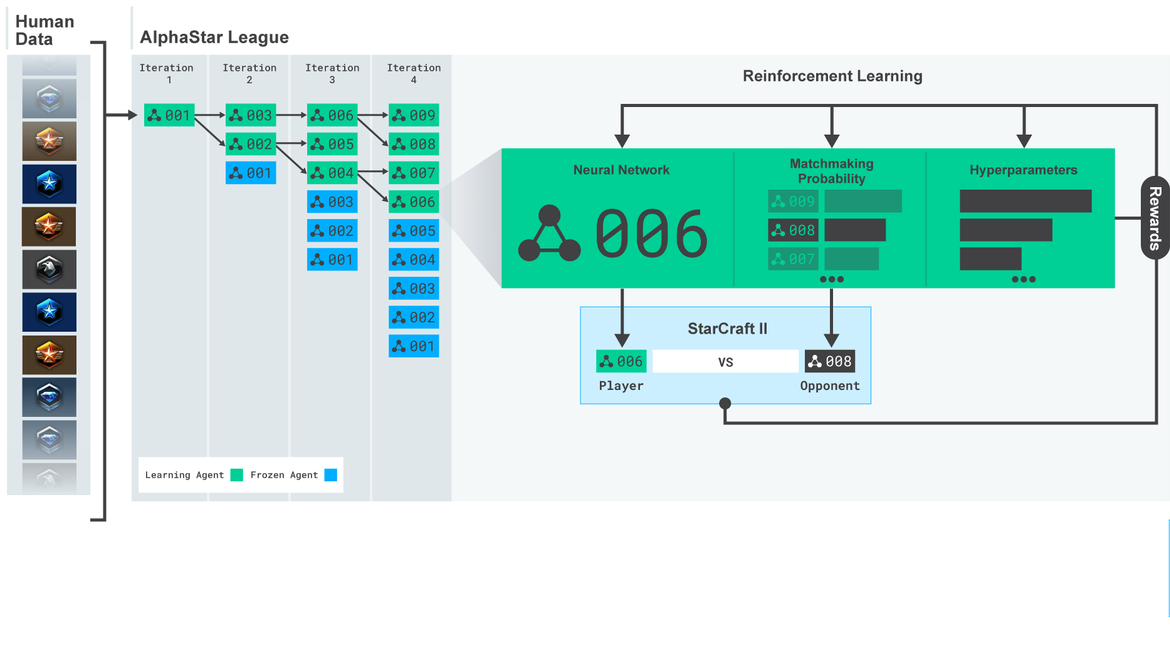
\includegraphics[scale=0.17]{images/SCII.png}
		\end{columns}
	}
\end{frame}

\end{document}